\newcommand{\R}[1]{\ensuremath{\mathbb{R}^{#1}}}
\newcommand{\DB}{\ensuremath{\mathcal{D}}}
%comandos para as variaveis


\chapter{Trabalhos Relacionados e Fundamentos}
\label{cap-trab-relacionados}

\section{Introdução}

Neste capítulo serão apresentados os fundamentos, métodos relacionados e conceitos teóricos necessários para o desenvolvimento deste trabalho bem como trabalhos relacionados mais relevantes....

A seção x trata de.......
%Colocar os topicos do que será dito

\section{Visualização de Informações}

Visualização de Informações é uma área de aplicação de técnicas de computação gráfica, geralmente interativas, visando auxiliar o processo de análise e compreensão de um conjunto de dados, através de representações gráficas manipuláveis\cite{gershon1998information}, é o processo de transformação de dados, informação e conhecimento em formas visuais em interfaces eficazes representando grandes volumes de dados a serem interpretados com mais rapidez e eficácia  descobrindo-se características ocultas, padrões ou tendências dificeis de se visualizar olhando os dados brutos\cite{gershon1998information} , normalmente provindos de  informações mais abstratas (que não possuem informações intrínsecas de geometria), tais como: documentos, textos, dados financeiros, informações de comércio, categorias e classificações, e conceitos não muito bem definidos.\cite{vaz2004visualizacao}

colocar uma imagem.

Ela é caracterizada pela necessidade do projetista de criar uma forma para transformar dados em uma representação gráfica. Esta representação deve expressar importantes propriedades dos dados e expressar como diferentes itens estão relacionados entre si. Portanto, todas as técnicas procuram representar, em gráficos ou figuras, informações que tentam explorar ao máximo a capacidade de percepção humana, levando à interpretações mais concretas e compreensíveis. \cite{vaz2004visualizacao}

Uma técnica de visualização é baseada numa representação visual e em mecanismos de interação que possibilitam ao usuário manipular essa representação de modo a melhor compreender o conjunto de dados ali representado \cite{freitas2001introduccao}. O nível de abstração dessa representação é mais alto, porque freqüentemente não há relação direta entre os dados e uma entidade física ou geométrica, ou o usuário não está interessado em dados brutos, mas em observar características ou padrões no conjunto de dados. 

Normalmente dados provindos dessas fontes tem mais de uma dimensão, cada instancia é a representação de um objeto, como uma pessoa, ela tem varias informações, como: nome, idade, altura, cor da pele, endereço, CPF, entre outros,  cada um desses dados representa uma dimensão 

\section{Visualização de Dados Multidimensionais}
\label{VisMultidimensionais-sec}

Para a percepção humana, os dados devem ser representados num espaço de baixa dimensão, normalmente em duas ou três dimensões. O objetivo dos métodos de visualização é a de representar os dados multidimensionais em um espaço de baixa dimensão de modo que determinadas propriedades (por exemplo, aglomerados de outliers) e a estrutura do conjunto de dados sejam preservadas o mais fielmente possível. Tal visualização é muito importante na mineração dos dados, porque as aplicações recentes produzem uma grande quantidade de dados que exigem meios específicos para descoberta de conhecimento.
Os métodos de redução de dimensionalidade ou visualização são técnicas recentes para descobrir o conhecimento escondido em conjuntos de dados multidimensionais. \cite{dzemyda2013multidimensional}

Na visualização são definidos por dois termos principais: objeto e funcionalidade. O termo objeto pode cobrir várias coisas: as pessoas, equipamentos, produtos de fabricação, plantas, fenômenos naturais, etc. Um objeto é caracterizado por algumas características. Por exemplo, o paciente é um objeto, ele (ela) pode ser descrita por um certo número de características, tais como nome, sexo, idade, e os resultados de teste de diagnóstico, como pressão sanguínea, nível de colesterol, etc. \cite{dzemyda2013multidimensional}


As fontes de dados aumentam substancialmente, tanto em tamanho como em complexidade, assim extrair informações úteis a partir delas torna-se um desafio. Uma medida de complexidade de dados é o número de atributos associados a cada instância de dados. Considere, por exemplo, dados de um censo demográfico: a instância de dados registra atributos, tais como idade, sexo, educação, ocupação, renda, etc. Considerando-se atribuir cada dado como uma dimensão de dados, se tivermos \textbf{m} tais atributos, cada instância de dados pode ser interpretada como um vector \textbf{m-dimensional} colocado num espaço de definição \textbf{m-dimensional}\cite{paulovich2008least}

Na análise estatística tradicional, os dados de instâncias com quatro ou mais dimensões são conhecidas como dados multivariados ou hipervariados. Texto por exemplo é um tipo de dado multidimensional. Os métodos convencionais para a visualização de dados multidimensionais, tais como gráficos de dispersão, coordenadas paralelas, ou métodos orientados a pixel, que são normalmente utilizados para auxiliar a interpretação dos dados, pode falhar se eles são aplicados diretamente a dados de alta-dimensional. Além disso, a identificação de padrões e modelos se torna mais difícil à medida que dimensionalidade aumenta (a maldição da dimensionalidade), e a falta de representações adequadas pode prejudicar gravemente a interpretação \cite{paulovich2008least}.

Uma forma comum de lidar com dimensionalidade é reduzir o número de dimensões de modo que as estratégias que são conhecidas que funcionam bem com dados de baixa dimensão podem ser aplicadas.  



\section{Técnicas de Projeção Multidimensional}

Técnicas de projeção multidimensionais são baseadas em combinações lineares de atributos de dados, definindo-os numa nova base ortogonal de pequena dimensão, ou em um processo que tenta minimizar uma função da perda de informação efetuadas durante a projeção. 

Técnicas lineares podem deixar de captar os padrões relevantes de dados com estruturas não-lineares, tais como clusters. Nesse caso, técnicas de minimização são melhores candidatas. No entanto, eles podem ser computacionalmente dispendioso para alcançar projeções de alta precisão. Assim, técnicas de projeção mais rápidas que podem capturar relações não lineares deve ser procurado.

Uma técnica de projeção multidimensional tipicamente mapeia os dados para um espaço com d dimenções, com d = {1,2,3}, continuando a manter no espaço projetando alguma informação sobre a relação de distância entre os itens de dados em seu espaço de definição original. Utilizando uma representaçoões gráficas unidas com a capacidade visual human
a de reconhecimento de padrões com base na similaridade de grupos de elementos.

A maioria das técnicas  que chamam a sua visualização a partir de dados extraídos (tais como citação, cocitação, de autoria, e palavras-chave).Projeções bem construídas podem ser usadas neste para exibir a estrutura global, subjacente ou tendências locais de uma coleção de documentos através da organização de semelhança em conteúdo com as regiões vizinhas no mapa. Conjuntos de dados textuais se tornam representações vetoriais com alta dimensionalidade e dispersão, tornando a aplicação particularmente difícil de ser processada com com algumas técnicas de visualização. Técnicas construídas para processar coleções de documentos extremamente grandes perdem muita informação quando procuram escalabilidade. Técnicas precisas são úteis para aplicações onde os usuários têm como objetivo examinar uma grande quantidade de documentos, mas são muito lentos, mesmo para conjuntos de dados de tamanhos moderado.


Formalizando o conceito de projeções multidimensionais baseadas na distância, tendo  $x={x_{1}, x_{2},...,x_{n}}$ como um conjunto de dados m-dimensional, com $\delta (x_{i},x_{j})$ sendo uma medida (distância) de dissimilaridade entre duas intâncias m-dimensionais de dados, e tendo $Y=(y_{1},y_{2},...,y_{n})$ como um conjunto de pontos em um espaço d-dimensional, com $d=\{1,2,3\}$ e $d=(y_{i},y_{j})$ sendo a distância (euclidiana) entre dois pontos do espaço projetado. Uma técnica de projeção multidimensional pode ser descrito como uma função injetiva $f : X\rightarrow Y$ que procura fazer $|\delta (x_{i}, x_{j})-d(f(x_{i}),f(x_{j})|$ o mais próximo possível de zero.

\section{Visualização Multidimensional na Web}



%-----------------------------------
\section{Visualização de Documentos e Textos}
\label{Visualizacao_texto}

Documentos ou textos podem ser extraídos de diversas fontes como \emph{blogs}, \emph{wiki}, conteúdo de \emph{twittes}, paginas da \emph{web}, conteúdo de livrarias digitais\cite{ward2015interactive}, artigos ciêntificos entre outros. Ward et. al. (2015)\cite{ward2015interactive} definem o conjunto dessas informações como \emph{corpora}.  Este \emph{corpora} contém objetos que podem ser compostos por palavras, frases, paragráfos, documentos e coleções de documentos \cite{ward2015interactive}.

Para que o texto seja consultado são feitos cálculos que definem a relevância da relação entre documentos relativos a uma determinada consulta pré-processada dos documentos e a interação semântica do texto \cite{ward2015interactive}. Em \cite{ward2015interactive} é definido três tipos de representações textuais: as léxicas, sintáticas e semânticas: 

Representações \textbf{léxicas} lidam com a parte da transformação de uma série de carácteres em uma sequência de entidades atômicas, chamadas de \emph{tokens}(marcadores), que definem regras para a sequência de símbolos. 

Representações \textbf{sintáticas} tratam da identificação e etiquetagem de cada \emph{token}. Podem ser atribuidas varias etiquetas, tais como a posição da sentença, ou se uma palavra é um substantivo, palavrão, adjetivo, palavra ambigua, ou uma conjunção \cite{ward2015interactive}. 

Já as representações de nivel \textbf{semântico} englobam a extração do significado e as relações entre pedaços do textos derivados de estruturas identificadas no nível sintático. Neste nível é definida uma interpretação analítica do texto completo dentro de um contexto específico, ou mesmo independente do contexto \cite{ward2015interactive}.

\emph{Tokens} também podem conter atributos como singular, plural, ou sua proximidade com outros \textit{tokens}, entre outros atributos \cite{ward2015interactive}.
 A riqueza e variedade de modelos de linguagem e gramáticas (generativo, categórica, a dependência, probabilística, e funcionalista) produzem uma ampla variedade de abordagens.

%O processo de extrair essas anotações é chamado reconhecimento de entidade nomeada (NER).

Além dessas informações contidas nos documentos eles podem conter metadados como nome do autor, data de criação, data de modificação, cometários ou tamanho \cite{ward2015interactive}.

Essas informações podem gerar visualizações dos mais variados tipos, dependendo da finalidade aplicação

%fazer a ligação com o proximo topico


\section{O Processo de Visualização}

O processo de visualização engloba todas as fases da visualização composta por quatro estágios básicos definidos por \cite{ware2012information}, combinados em certo número de laços que se repetem até chegar ao nível de informação necessário.

Os quatro estágios são: A \textbf{coleta e armazenamento de dados}.  
O \textbf{pré-processamento} concebido para transformar os dados em algo que podemos entender. O \textbf{hardware} de exibição e os \textbf{algoritmos} gráficos que produzem uma imagem na tela.
O sistema perceptivo e cognitivo humano (\textbf{o observador/usuário}).

O ciclo mais longo envolve a coleta de dados, pois, os dados podem chegar de maneira costante tendo que se atualizadar a base de dados e a visualização. 

Outro ciclo controla o pré-processamento computacional que ocorre antes da visualização.
Dependendo do tipo de dados tanto o ambiente físico e do ambiente social estão envolvidos no ciclo de coleta dos dados. O processo de criação da visualização é demostrado na figura \ref{fig:processovisual}.

\begin{figure}[htb]
		\begin{center}
			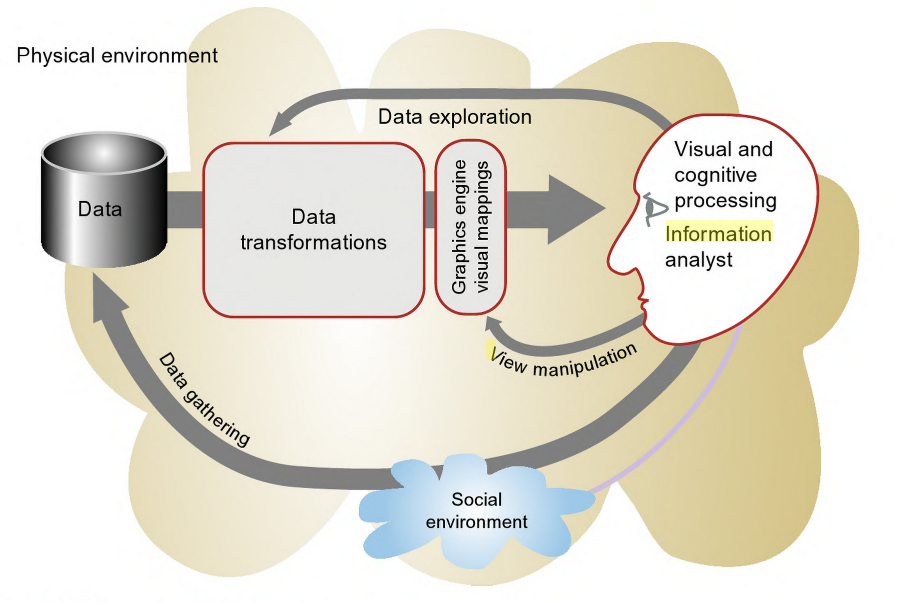
\includegraphics[width=13cm]{images/LevelVisualization.png}
            \caption {Estrutura do processo de análise visual \cite{ware2012information}.}          
            
	\label{fig:processovisual}
		\end{center}
	\end{figure}

O computador é tratado,  como uma ferramenta para a produção de gráficos interativos. Isto significa que uma vez descoberta a melhor maneira de visualizar os dados para uma determinada tarefa, podem ser desenvolvidos algoritmos para criação de visualizações apropriadas.

A questão crítica é qual a melhor forma de transformar os dados em algo que as pessoas possam entender para a melhor tomada de decisão\cite{ware2012information}.

Para o processo de desenvolvimento, além da visualização representar o conjunto de dados, é importante que sejam exploradas funcionalidade que permitam, não somente a interpretação correta dos dados, mas também um mecanismo eficiente para a geração de conhecimento, de modo que as análises sejam realizadas de forma automática simplificando a compreensão \cite{keim2006challenges}. Aliado a isso, é necessário explorar, da melhor forma possível, os recursos disponíveis, para que sejam desenvolvidas técnicas visuais que realmente auxiliem e facilitem a interpretação dos dados \cite{keim2006challenges}.

%fazer ligação com o proximo tópico


\section{Projeções Multidimensionais}
\label{Projecoesmultidimensionais}


dfsd

\section{Controles da interação}

Para que o usuário possa acessar as informações de maneira mais prática é preciso alguns mecanismos de controle de interação, como escolher o tipo de visualização, localização e nível de cada interação navegando dentro dos dados e da visualização \cite{ward2015interactive}. Controles devem ser intuitivos sem ambiguidades e com nível de detalhamento e precisão adequadas para o espaço em que estão sendo operados\cite{ward2015interactive}. 

\section{Técnicas de Ranqueamento}

\textit{PageRank} é um algoritmo de ranqueamento comumente utilizado para ranqueamento de páginas \textit{web}. Ele explora a estrutura do hipertexto de uma página para representar associações e a partir daí quantificar e propagar a importância de determinado página pela web \cite{langville2011google}.
O algoritmo faz a exploração da seguinte maneira: Uma página A que possui um \textit{link}, ou referência, para uma página B, é contado como um ponto para a página B. Entretanto, não apenas essa informação é levada em consideração, mas também a pontuação ou importância das páginas que referenciaram B, neste caso, o escore da página A influencia no escore da página B \cite{de2006mecanismos}. 
Para documentos será aplicado o mesmo fundamento, se um documento X refererencia um documento Y este documento tem um ponto, cada referência a mais soma-se mais pontos, além disso o número citações do artigo X influência na relevância do artigo Y, no final quanto maior do artigo pontuação maior será a sua relevância em relação aos documentos na base.

\begin{figure}[htb]
		\begin{center}
			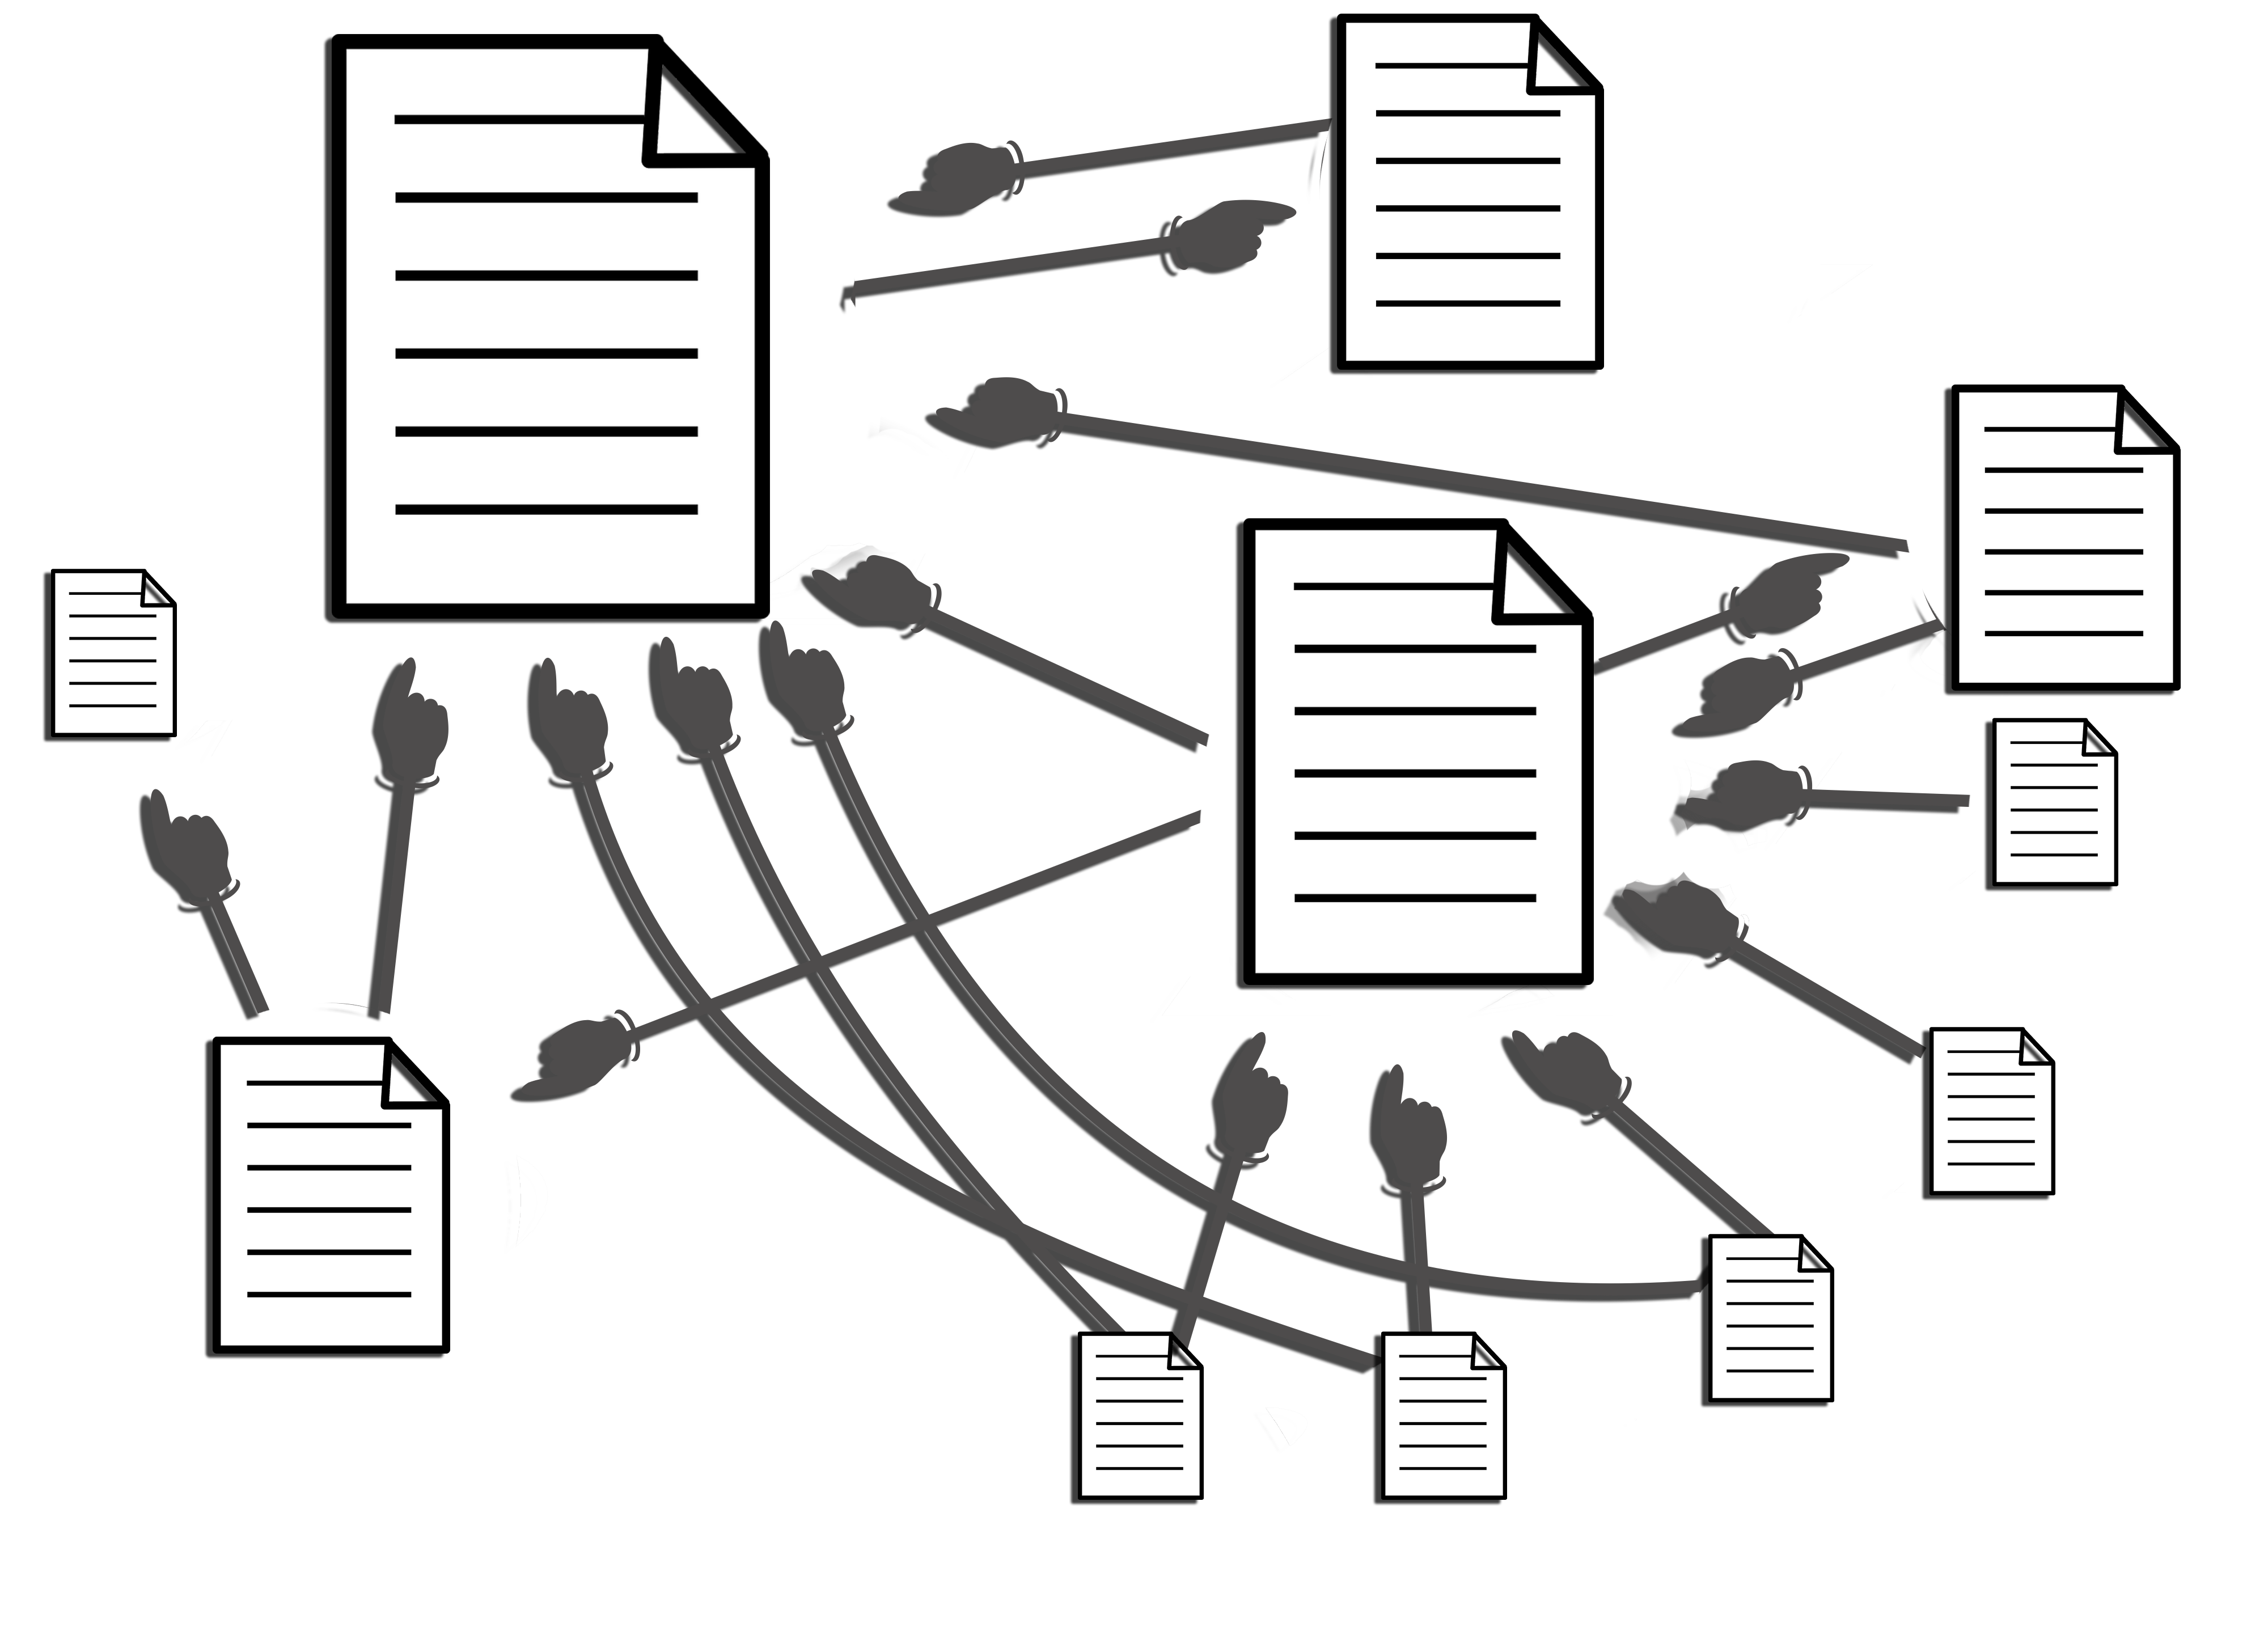
\includegraphics[width=13cm]{images/pagerankgex.png}
            \caption{Modelo simplificado do algoritmo \textit{PageRank}}
            %\cite{pagliosa2013mist}
            
	\label{pagerankfig}
		\end{center}
	\end{figure}



\section{Conceitos e Ferramentas Web}

Uma aplicação Web típica é um sistema computacional distribuído cliente-servidor. A parte servidor da aplicação é responsável por receber e processar solicitações de um cliente, comumente enviadas através de um navegador Web. O resultado do processamento efetuado pelo servidor é uma página Web, a qual é enviada de volta ao cliente e então exibida no navegador. O conteúdo de uma página Web (textos, imagens, links,controles, etc.) é definido por elementos descritos em Hypertext Markup Language (HTML), cuja versão mais recente é HTML5 (WANG; FRANK; MOSKOVITS, 2013). Além disso, uma página Web pode usar arquivos Cascate Style Sheets (CSS) (W3C, 2014a) para definir localização, cor, estilo, etc. de seus elementos,
caracterizando assim a aparência e o leiaute da página.

	
\subsection{D3}

D3 (Data Driven Document) é uma biblioteca para manipulação de documentos com base em dados dinâmicos que permite a criação de gráficos manipulaveis fazendo associoação entre eles \cite{d3site} \cite{zhu2013data}.  É  uma peça de software que facilita a geração e manipulação de documentos web com dados usando HTML, SVG e CSS \cite{murray2013interactive}. O foco desta biblioteca são padrões web, combinando componentes de visualização com uma abordagem de manipulação de elementos baseada em DOM\cite{d3site} . Com D3 é possível criar aplicações variadas \cite{d3site}, desde gráficos simples até mais complexos, como  box splots interativos, grafos com força direcionada, aplicações com detecção de colisão, entre outros exemplos mostrados na figura \ref{fig:d3exemplos},  entre outras. 

\begin{figure}[!ht]
	\centering
	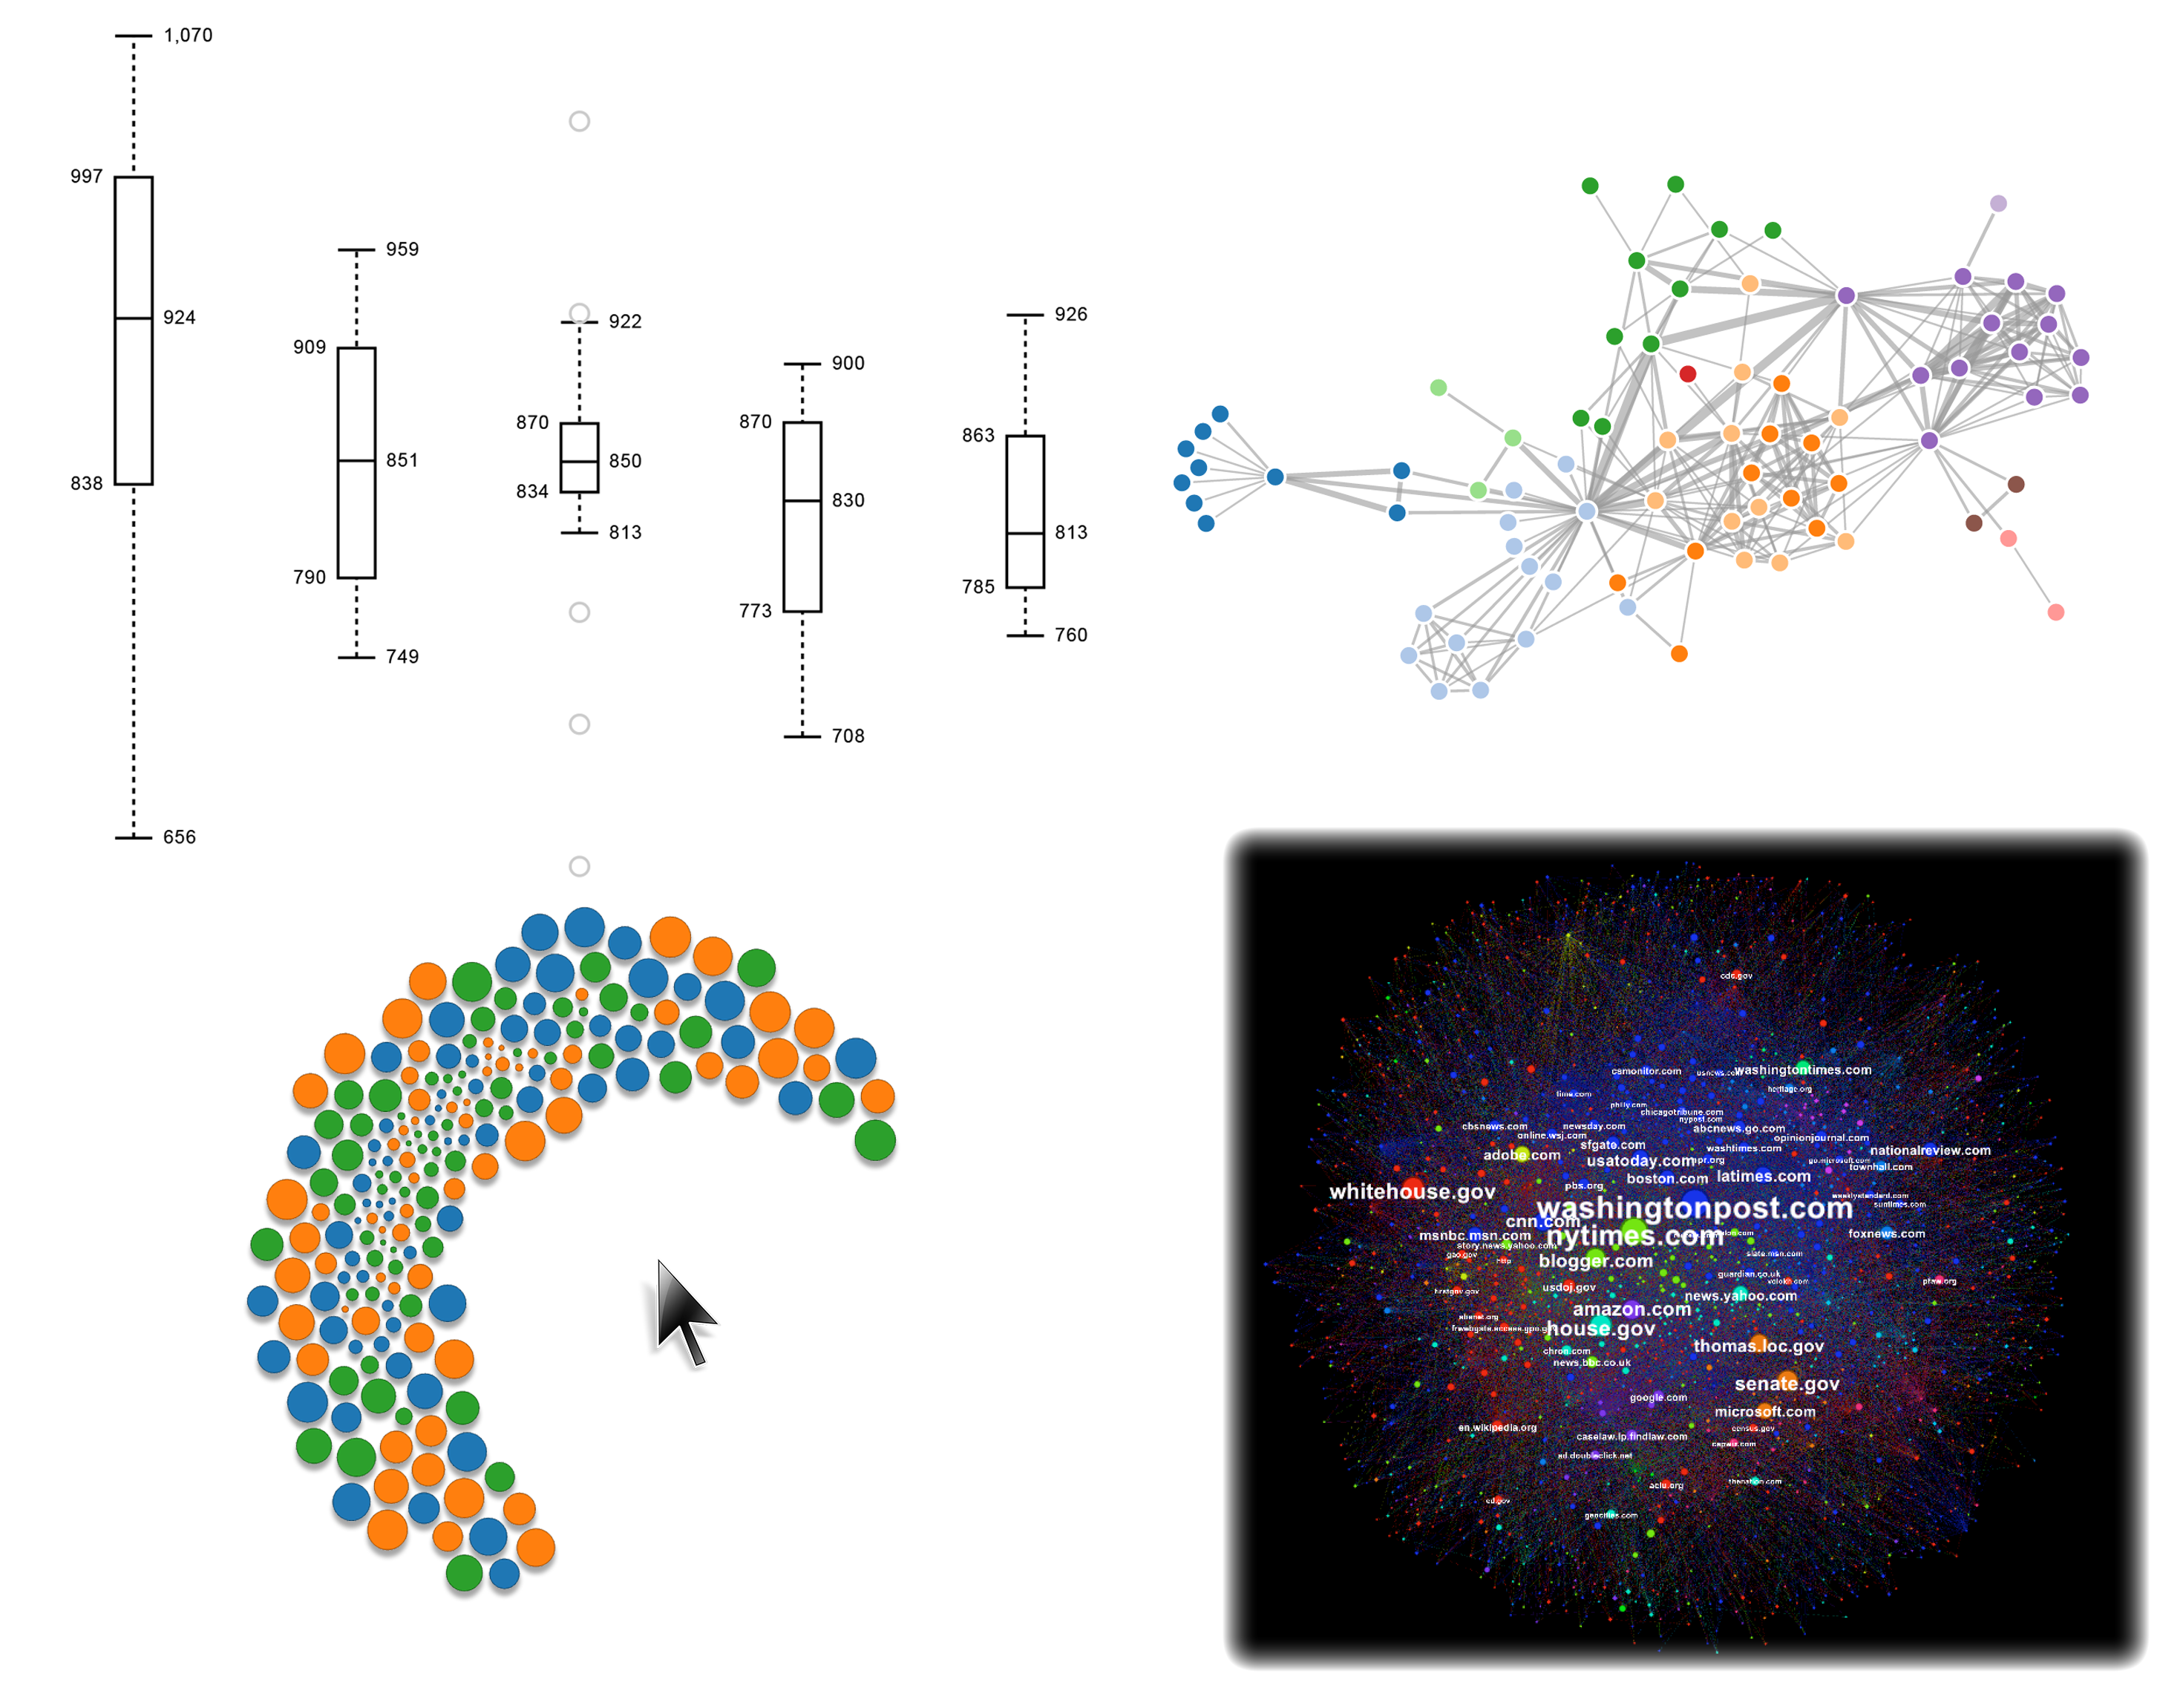
\includegraphics[width=1\columnwidth]{images/D3jsexemplos.png}
	\caption{Exemplos de visualização com D3  \cite{d3site}}
	\label{fig:d3exemplos}
\end{figure}

........

\subsection{jQuery}

Outra biblioteca que sera usada a jQuery que é uma biblioteca JavaScript rápida, pequena e rica em recursos capaz de adicionar interatividade e dinamismo às páginas web com objetivo de fazer isso de forma simplificada \cite{bibeault2008jquery}. Ela é multi plataforma e \textit{open source}\cite{bibeault2008jquery}, foi criada dentro dos Padrões Web estipulados pela W3C, por este motivo é uma biblioteca multi-plataforma, ou seja, é compatível com qualquer navegador de internet.

jQuery, em sua essência, é uma biblioteca de manipulação de DOM (Document Object Model) \cite{duckett2014web}. O DOM é uma representação em árvore-estrutura de todos os elementos de uma página Web e o jQuery simplifica a sintaxe para encontrar, selecionar e manipular esses elementos DOM \cite{bibeault2008jquery}. O jQuery também fornece recursos para os desenvolvedores criarem plug-ins sobre a JavaScript \cite{duckett2014web}. Isso permite aos criar abstrações para interações de baixo nível, animação, efeitos avançados de alto nível, e widgets personalizáveis. A abordagem modular para a biblioteca jQuery permite a criação de poderosas páginas web dinâmicas e aplicativos Web.




\section{Trabalhos Relacionados}
\label{Trab_Relac}


O MIST \textit{(Multiscale Information and Summaries of Texts)} é uma ferramenta que permite a visualização simultânea de documentos individuais, bem como um resumo do conteúdo de coleções de documentos, permite uma exploração multi escalar de subconjuntos de documentos por conteúdo\cite{pagliosa2013mist}. 


\begin{figure}[!ht]
	\centering
	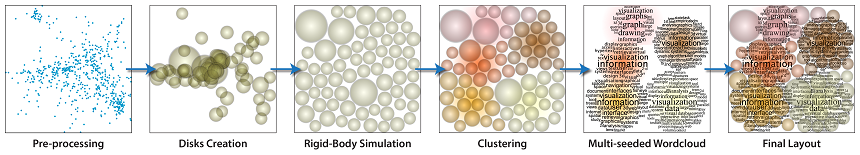
\includegraphics[width=1\columnwidth]{images/mist_pipeline.png}
	\caption{Pipeline de visualizações do MIST \cite{pagliosa2013mist}}
	\label{fig:MISTpipeline}
\end{figure}

A técnica MIST compreende três etapas principais: pré-processamento, criação de discos, simulação de corpo rígido e geração de nuvem de palavras, como ilustrado na Fig. \ref{fig:MISTpipeline}. Três tarefas são realizadas durante o pré-processamento. A primeira tarefa é um processo de extração de palavras-chave, para gerar a nuvem de palavras no terceiro passo do pipeline. Palavras-chave são também usadas para calcular a similaridade entre documentos. Esta semelhança é usada no segundo passo, como entrada para um processo de projeção multidimensional que mapeia os documentos em um espaço visual 2D. A importância de cada documento na coleção também é computada como uma pré-tarefa de processamento e é baseada na ligação entre os documentos individuais, dadas por um usuário ou aplicação definida. Na segunda etapa do MIST, uma simulação de motor de corpo rígido  organiza um conjunto de discos que representam os documentos, com o seu tamanho determinado pela importância do documento, evita também sobreposições e ainda preserva estruturas de vizinhança fornecidas pela projeção multidimensional inicial \cite{pagliosa2013mist}.
Na terceira e última etapa do pipeline, os documentos são agrupados de acordo com sua vizinhança, após isto, nuvens de palavras são geradas e harmoniosamente fundidas para produzir o layout final.

 Mas, a aplicação tem limitações como por exemplo a quantidade de artigos que podem ser processados (\textit{deadline:} 2 mil artigos), não sendo viável tratar uma quantia maior de artigos, entre outras que serão exploradas ao decorrer do trabalho. Para que a ferramenta seja usada para processar uma quantia maior de artigos terá de ser feita uma reestruturação de seus algoritmos e métodos.

Contexto e relevância (o que já existe atualmente: MIST).

Lacunas do MIST a serem investigadas no projeto:
\begin{itemize}
	\item Tamanho da base de dados \DB\ pode se tornar ``grande''. Como consequência, à medida que novas instâncias são adicionadas a \DB,
	tornam-se necessário o uso de um método de ranqueamento e de projeção
	multidimensional \emph{incrementais}. Atualmente, MIST emprega
	projeções que podem manipular somente conjuntos ``pequenos'' de
	dados.
	
	\item MIST não admite consultas iniciais.
	
	\item As formas geométricas em MIST são restritas a círculos.
	
	\item O método de repulsão é baseado em impulsos aplicados às formas
	geométricas, consideradas como sendo corpos rígidos
	bidimensionais. O método não consegue fazer uma escala eficiente para um número
	``grande'' de pontos.
	
	\item MIST não emprega uma metáfora para densidade de pontos.
	
	\item MIST não efetua agrupamentos no espaço \R{m}, mas sim no
	espaço visual \R{2}. O número de grupos é especificado
	arbitrariamente pelo usuário e computado através de
	\emph{k-means}. Como consequência, as instâncias em um agrupamento
	não mantêm necessariamente outra relação entre si que não seja a de
	proximidade de suas projeções no espaço visual.
	
	\item MIST sumariza um agrupamento através de nuvens de palavras, as quais são exibidas como textura de fundo do retângulo envolvente do agrupamento no espaço visual. Tal procedimento restringe o emprego	de sumários. Embora a visualização contenha vários elementos
	informativos, pode-se contestar a real eficácia de tal esquema de	sumarização, além da confusão visual por parte de usuários.
	
\end{itemize}


\section{Outros Trabalhos}

Koh et. al. \cite{koh2010maniwordle} apresentam uma ferramenta de visualização de palavras baseada em \textit{Wordle} (aplicação usada para gerar nuvens de palavras) o \textit{ManiWordle}. Ele renova as interações com o \textit{layout}, apoiando manipulações personalizadas, permite a manipulação de tipografia, cor e composição, não só para o layout como um todo, mas, também para as palavras individuais, permitindo ter um melhor controle sobre o resultado do \textit{layout}. 

Wu et. al. \cite{xu2016semantic} descrevem um método para criar nuvens de palavras preservando a relação semântica, formando um gráfico de semelhança entre as palavras  de acordo com a distância sêmantica. Métodos, como \textit{SparkClouds} apresentado em \cite{lee2010sparkclouds} e \textit{Tag Clouds Paralel} \cite{collins2009parallel}, aumentam as nuvens de palavras com recursos visuais adicionais, tais como linhas de ignição e coordenadas paralelas, a fim de melhor transmitir o conteúdo do resumo de documentos.  Embora muito eficazes para descobrir informações essenciais contidas em uma coleção de documentos, o paradigma da nuvem de palavras por si só não identifica a associação entre palavras para um determinado documento ou grupo de documentos e não permite o exame de similaridade entre eles. 

Árvore de palavras é uma técnica de visualização que representa tanto a frequência do termo como o contexto. Comumente o tamanho da palavra representa a frequência em que a palavra ou frase ocorre o texto.  A raiz da árvore é uma palavra ou frase de interesse especificado pelo usuário, e os ramos representam os diferentes contextos em que a palavra ou frase é usada no documento \cite{ward2015interactive}.

O \textit{WordTree} \cite{wattenberg2008word} é um exemplo do uso desta técnica, ele cria uma árvore com nós representando termos e ramos que ligam termos sequenciais, chamada de "árvore de sufixo". É possivel a navegação em um texto selecionando uma palavra ou grupos de palavras, e verificar todas as sentenças que os incluem, permitindo consultas exploratórias rápidas. o \textit{Phrase Nets} \cite{van2009mapping} é outro que emprega um \textit{layout} baseado em gráfos onde os nós (\textit{nodes}) correspondem a um subconjunto de palavras e as arestas correspondem à relação semântica ou léxica entre as palavras. O tamanho da fonte e espessura de borda são usados para mapear visualmente os atributos como o número de ocorrências de um conjunto de palavras e seus relacionamentos. 

Uma análise linguística mais sofisticada é aplicada pelo \textit{DocuBurst} \cite{collins2009docuburst}, ele faz uso de uma base de dados léxica eletrônica e um \textit{layout} de árvore com preenchimento radial no espaço para visualizar o conteúdo do documento de uma forma léxica. Keim e Oelke \cite{keim2007literature} desenvolveram um método que emprega regras semânticas para segmentar um documento em blocos e funções de palavras para mapear os blocos em vetores de características. O principal componente de cada recurso do vetor é usado para colorir os blocos, resultando em uma imagem como uma impressão digital do documento. Em contraste com os outros métodos  baseados em linguística acima descritos, o método de Keim e Oelke \cite{keim2007literature} permite identificar e comparar os documentos específicos no conjunto de dados, mas, comprometem a legibilidade do seu conteúdo.


Em \cite{joia2015uncovering} é proposta uma técnica de visualização multidimensional com projeção que se baseia em exemplos representativos para definir agrupamentos no espaço visual. Exemplos representativos são selecionados por um sistema de amostragem determinista derivada da decomposição da matriz que é sensível à variabilidade de dados capaz de lidar com as classes com um pequeno número de casos. Além disso, o mecanismo de amostragem pode facilmente ser adaptado para selecionar atributos relevantes de cada agrupamento.

Um mecanismo muito eficiente para visualizar variações temáticas de coleções de documentos em uma linha do tempo são as metáforas de rio (River Metaphor). Com essas metáforas pode-se visualizar variações nos estilos comparando com outros documentos através de uma linha do tempo oriundas de eventos externos. Introduzido inicialmente pelo sistema ThemeRiver \cite{havre2002themeriver}, as metáforas foram melhoradas com mecanismos sofisticados para fazer a derivação em relação aos tópicos de detecção de tempo \cite{liu2012tiara} e visualizações em camadas capazes de descrever o nascimento, morte e divisão de classes de eventos \cite{cui2011textflow}. 

Há também o EventRiver \cite{luo2012eventriver} que faz uso de um esquema de \textit{cluster} para grupos de notícias similares que tenham conteúdos próximos ao longo do tempo, como colunas de jornal, ele usa metáfora de bolha cuja espessura representa o número de documentos, o comprimento e a duração de um evento. Em  \cite{viegas2004studying} é apresentada uma ferramenta para fazer uma análise exploratória de dados, o fluxo histórico de visualização, também pode ser visto como metáfora de rio concebido para visualizar edições de um documento (ou uma coleção de documentos, tais como a Wikipédia) que é feito por diferentes autores, enfatizando partes que sobrevivem ao longo do tempo. Metáforas de rio proporcionar uma visualização agradável e intuitiva quanto ao comportamento temporal de uma coleção de documentos, mas, semelhante a nuvens de palavras, a técnica não permite a identificação imediata de documentos específicos, a sua relevância dentro da coleção ou a sua contribuição para um tópico. Além disso, interagir com o esquema de rio para realizar alterações na perspectiva do usuário não é viavel.



Existem algumas técnicas que se baseiam em estruturas hierárquicas, elas permitem um nível de detalhamento, exploração e navegação diferente das demais apresentadas encontradas na literatura. Topic Island \cite{miller1998topic}, por exemplo, cria uma hierarquia através da aplicação de uma transformada \textit{wavelet} em sinais customizados extraídos de palavras do documento. A hierarquia permite a visualização com alterações de tema e partes importantes da coleção de documentos relacionados com o conteúdo total do documento.
InfoSky \cite{andrews2002infosky} visualiza documentos hierarquicamente organizados, subdividindo o espaço visual usando um diagrama de Voronoi recursivo. A navegação em toda a hierarquia é ativada por um mecanismo tipo um zoom telescópico. Hipp \cite{paulovich2008hipp} faz uso de um conjunto de árvores para organizar hierarquicamente documentos de acordo com a sua semelhança, o resultado da visualização é uma árvore. 

Mao et al.\cite{mao2007sequential} apresentam uma técnica para visualizar documentos usando curvas construídas a partir de uma generalização de \emph{n-grams} e médias locais, a construção da hierarquia, alterando o apoio dos grãos usados no cálculo da média. Embora eficaz para construir sumarizações visuais, bem como para identificar as estruturas nos tópicos do documento, técnicas hierárquicas não são eficazes para associar conteúdo e documentos quando a hierarquia é feita sobre os temas. Além disso, a visualização da estrutura hierárquica exibida simultaneamente à importância de cada documento, não é uma tarefa simples \cite{pagliosa2013mist}.

 Em \cite{oesterling2014topology} é proposto um método baseado em topologia que evita a oclusão estrutural para preservar recursos de agrupamentos primários e propriedades geométricas negligênciadas que não podem ser preservadas em representações de baixa dimensionalidade. Ele abstrai os pontos de entrada nas regiões com as propriedades de cada um e fornece ao usuário visualizações intuitivas tipo paisagem que ilustram a estrutura de alta dimensão do agrupamento livre de oclusão.
 


\cite{bergstromeigenfactor}Eigen factor 

\cite{wesley2015static} Static ranking of scholarly papers using article-level eigenfactor

